\section*{1. Basic solar structure}

a) Draw an illustration diagram of the Sun with the following components and write a short description of
each component: solar wind, corona, chromosphere, photosphere, convection zone, radiation zone, core and
sunspots.\\
\noindent\makebox[\textwidth]{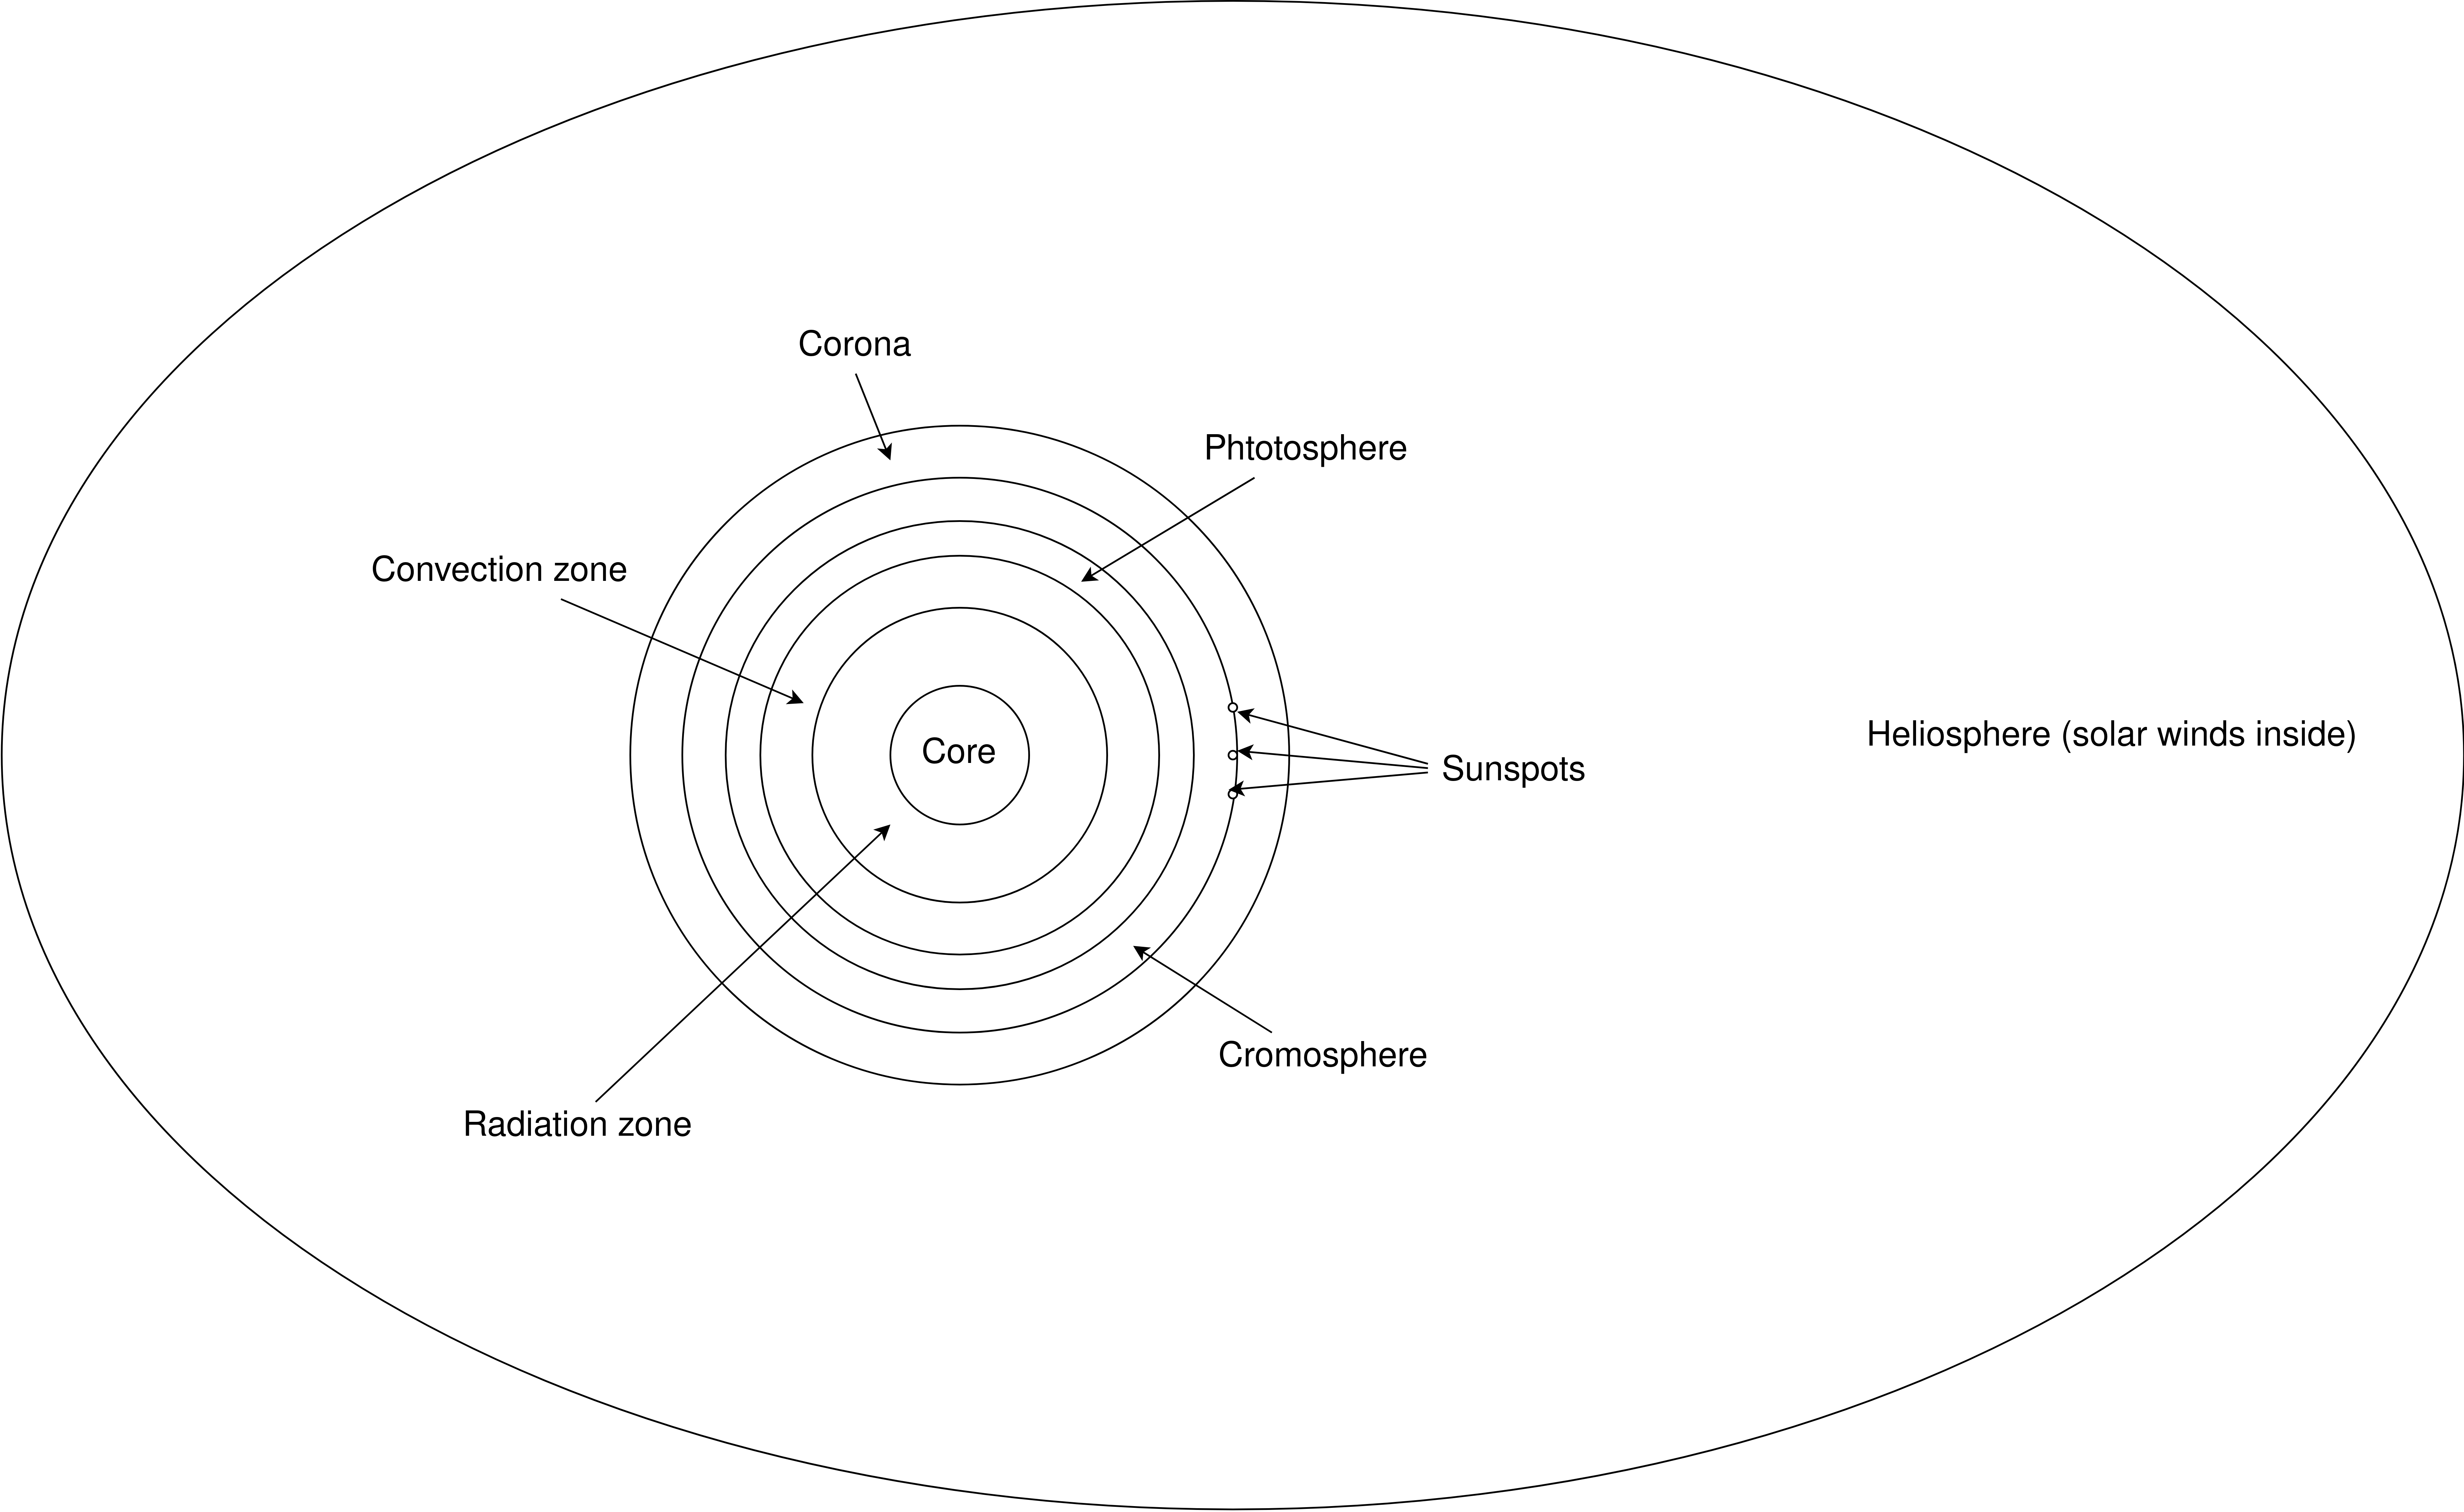
\includegraphics[scale=0.35]{sun.png}}
\noindent
\textbf{Solar wind} is a stream of charged particles, predominantly electrons and protons, ejected from 
the Sun's outer layers into space.\\
\\
\textbf{Corona} is the outermost layer of the Sun's atmosphere, characterized by extremely high 
temperatures. It can be seen as a halo during a solar eclipse.\\
\\
\textbf{Convection zone} is a layer of the Sun where heat is transported outward by the rising of hot 
plasma and sinking of cooler plasma. Energy transfer occurs through convection currents.\\
\\
\textbf{Radiation zone} is where energy is transported by electromagnetic radiation (photons) rather than 
the movement of material. Photons can take thousands to millions of years to travel from the core to the 
outer layers in this zone.\\
\\
\textbf{Core} is the central region of the Sun where nuclear fusion reactions occur. High temperatures 
and pressures enable hydrogen atoms to fuse into helium, releasing huge amounts of energy.\\
\\
\textbf{Chromosphere} is a layer of the solar atmosphere located just above the photosphere. It appears as
a red glow and is visible during a solar eclipse.\\
\\
\textbf{Photosphere} is the visible surface of the Sun that emits light and heat. It is the layer where 
most of the Sun's energy is radiated into space as sunlight.\\
\\
\textbf{Sunspots} are temporary phenomena on the Sun's photosphere that appear as dark spots. They are 
caused by magnetic activity and are cooler than their surroundings.\\
\\
b) Use Wien's Law to calculate the wavelength of peak thermal emission from the average temperature of the
surface of the Sun. What color does this correspond to? How does that compare to the color of the Sun that
the human eye perceives?\\
\\
c) The corona has a temperature of around 1 million K. How does this compare to the temperature of the
surface of the Sun?\\
\\

